\chapter{Techniques}

\section{Scanning Tunnelling Microscopy - STM}

The main technique used in this study is scanning tunnelling microscopy (STM), and more specifically the Aarhus STM. The Aarhus STM is an enhancement of the original version invented by Heinrich Rohrer and Gerhard Binnig in 1981.\cite{aarhusSTM} The STM is used to create surface images with atomic resolution of conducting samples, which makes the technique irreplaceable in this study.\\
\begin{wrapfigure}{r}{0.32\textwidth}
  \begin{center}
    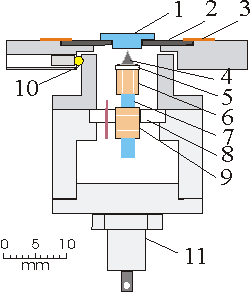
\includegraphics[width=0.32\textwidth]{aarhusSTM}
  \end{center}
  \caption{Schematic of the aarhus STM. \cite{aarhusSTM}}
  \label{aarhusSTM}
\end{wrapfigure}
Images of the sample surface are made from scanning the sample surface with a very sharp metal tip. As the sample is scanned, the tunnelling current between the tip and the sample is mapped, in order to create a topographical image of the surface. The high sensitivity of the STM stems from the tunnelling transmittivity which depends exponentially on the distance between the tip and the sample. The distance to the surface is measured indirectly by the tunnelling current which changes by about a factor of 10 for every ångstrøm.\cite{STMbinnig} A figure of the aarhus STM is shown in figure \ref{aarhusSTM}. The sample (1) is positioned within the Tantalum sample holder (2) and both are held tight by clamps(3). The STM tip held by a macor holder (5) is seen just above the sample (4) and this is controlled by the piezo scanner tube (6). In continuation of the scanner tube, a rod (7) is mounted which extends through another configuration of piezo elements abbreviated "The inchworm". This inchworm motor, held by another macor ring (8), is able to clamp to the rod and either expand or contract, in order to approach and retire the tip from the sample. The STM is thermally isolated from the rest of the environment by quartz balls (10). If the temperature drops during cooling despite the thermal isolation,  a zener diode (11) is mounted in order to heat the STM.\\
\\
At relatively large distances the barrier that the electrons perceive is too high, and no tunnelling occurs. As the distance between the sample and the tip is reduced the probability of an electron tunnelling through the vacuum barrier increases until a certain point where tunnelling happens, and the current can be measured. In order for any current to flow, a bias is required between the sample and the tip. This voltage difference ensures that the fermi level is raised in either the tip or the sample.


In order to create an image, the surface of the sample is scanned with the tip, which is moved by piezo-elements. The tunnelling current is dependant on distance between tip and sample as well as the local density of states (LDOS). A map of the LDOS is therefore obtained when the tip is scanned across the surface of the sample. This is used to indirectly create an image of the surface.\\

The tunnelling current can be calculated from first order pertubation theory. Here the individual wavefunctions of the tip and the sample are used as well as the potential barrier from the vacuum between the tip and the sample.

\begin{align}
  I = \frac{2\pi}{\hbar}e^2 V \sum_{\mu v}|M_{\mu v}|^2 \delta (E_v - E_F)\delta (E_{\mu}-E_F)
\end{align}

Here V is the applied voltage, $M_{\mu v}$ is the tunnelling matrix element between the states $\psi _{\mu}$ of the tip and $\psi _v$ of the surface and $E_{\mu}$ is the energy of state $\psi _{\mu}$ in the absence of tunnelling.

\section{Temperature Programmed Desorption - TPD}


\section{Low Energy Electron Diffraction - LEED}
